\documentclass{article}
\usepackage[T1]{fontenc}
\usepackage{lmodern}
\usepackage{graphicx}
\usepackage{amsmath,amssymb}
\usepackage[a4paper,margin=2cm]{geometry}
\usepackage[absolute,overlay]{textpos}
\setlength{\TPHorizModule}{1mm}
\setlength{\TPVertModule}{1mm}
\usepackage[indonesian]{babel}
\usepackage{hyperref}
\setlength{\emergencystretch}{2em}
% unit: Halaman 30

\begin{document}

% === Halaman 30 (llm) ===

\section*{1. Serangan pasif (passive attack)}

\begin{itemize}
    \item penyerang tidak terlibat dalam komunikasi antara pengirim dan penerima
    \item penyerang hanya melakukan penyadapan untuk memperoleh data atau informasi sebanyak-banyaknya
    \item enkripsi pesan mencegah penyadap memahami isi pesan
\end{itemize}

\vspace{10mm}

% deskripsi: Ilustrasi serangan pasif yang menunjukkan Alice mengirim pesan terenkripsi kepada Bob, sementara Eve bertindak sebagai penyadap (eavesdropper) yang mencoba mengintip komunikasi tersebut.
% bbox normalisasi: [0.2060, 0.5060, 0.8230, 0.8830]
\begin{textblock*}{129.57mm}(43.26mm,150.28mm)
\noindent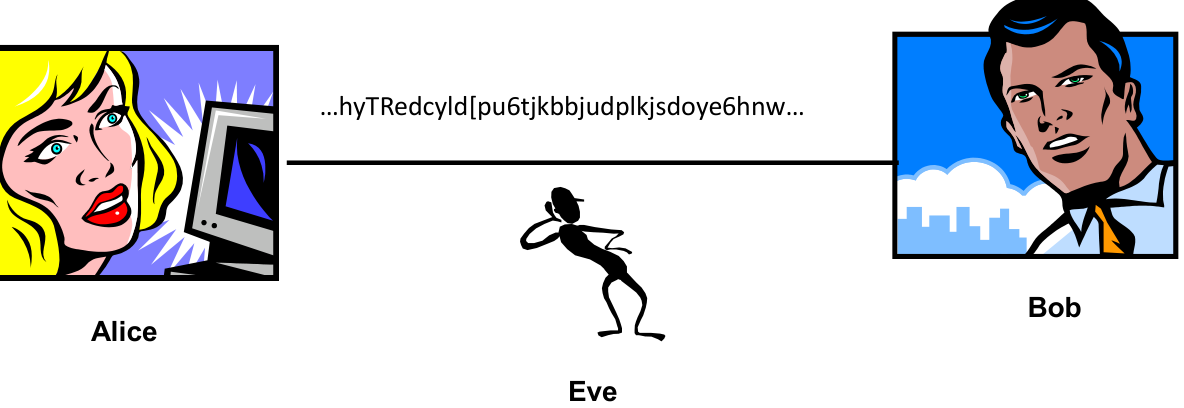
\includegraphics[width=129.57mm,height=111.97mm]{../../images/llm/page_030_img_01.png}%
\end{textblock*}

\end{document}
